\documentclass{beamer}

\usetheme{Frankfurt}

\usepackage{hyperref}

\AtBeginSection[] {
    \begin{frame}
        \frametitle{Table of Contents}
        \tableofcontents[currentsection]
    \end{frame}
}

\begin{document}

%%% title stuff
\title{An introduction to special relativity:}
\subtitle{a geometric approach}
\author{Nilay Kumar}
\date{January 9, 2014}
\frame{\titlepage}
%%% end title stuff

\begin{frame}
    \frametitle{Table of Contents}
    \tableofcontents
\end{frame}

\frame{\Large{Ask questions!}}

\section{History and development}
\subsection{The situation before 1900}

\begin{frame}
    \frametitle{The situation before 1900}
    \begin{itemize}
        \item Maxwell unifies electricity and magnetism, light is a wave
        \item Waves need a medium in which to propogate: ether
            \begin{itemize}
                \item negligible density and interaction with matter
            \end{itemize}
        \item Ether existed solely for E\&M
            \begin{itemize}
                \item Fizeau's experiments (1850's): ether must be dragged along by moving fluids according to $n$!
                \item Michelson-Morley (1886): no detected ether wind
            \end{itemize}
    \end{itemize}
\end{frame}

\begin{frame}
    \frametitle{Galilean transformations}
    \begin{block}{Observation}
        Newtonian mechanics is invariant under the Galilean transformations:
        \begin{align*}
            \mathbf{x'} &= \mathbf{x}-\mathbf{v} t\\
            t' &= t
        \end{align*}
    \end{block}
    \begin{itemize}
        \item This is not true of Maxwell's equations!
        \item Electromagnetic phenomena are instead Lorentz invariant
    \end{itemize}
\end{frame}

\subsection{Einstein's options}
\begin{frame}
    \frametitle{Einstein's options}
    \begin{enumerate}
        \item Maxwell's equations were incorrect; they must be adjusted to be invariant under Galilean transformations
        \item Galilean relativity applied to classical mechanics, but E\&M had a preferred reference frame given by the ether
        \item There existed a relativity principle for both mechanics and E\&M but it was not Galilean, implying that mechanics
            was in need of revision
    \end{enumerate}
\end{frame}

\subsection{Response and verification}

\begin{frame}
    \frametitle{Criticism and verification}
    \begin{itemize}
        \item SR was a radical shift in physical perspective
        \item Many physicists claimed that SR 
            \begin{itemize}
                \item was too abstract and mathematical
                \item did not agree with experiment
                \item was not interally consistent
            \end{itemize}
        \item Extensive testing:
            \begin{itemize}
                \item Michelson-Morley (isotropy), Kennedy-Thorndike (speed), Ives-Stillwell (time dilation)
                \item Multitude of more and more precise experiments
                \item Particle accelerators
            \end{itemize}
    \end{itemize}
\end{frame}


\section{The structure of SR}

\subsection{The two postulates}

\begin{frame}
    \frametitle{Postulate 1}
    \begin{block}{Postulate of relativity (Galileo)}
        The laws of nature and the results of all experiments performed in a given
        inertial frame of reference are independent of the translational motion
        of the system as a whole.
    \end{block}

    \begin{itemize}
        \item There is no absolute velocity!
        \item An inertial frame is an unaccelerated coordinate system for space and time that observes events as $(t,x,y,z)$ 
    \end{itemize}
\end{frame}

\begin{frame}
    \frametitle{Postulate 2}
    \begin{block}{Postulate of the constancy of the speed of light (Einstein)}
        The speed of light is finite and independent of the motion of its source
        or the motion of the inertial observer. In other words, two different
        inertial observers measuring the speed of the same photon will each find
        it moving at $c=3\times 10^8\text{ m/s}$ relative to themselves, regardless
        of the relative state of motion.
    \end{block}
    \begin{itemize}
        \item Completely invalidates Galilean addition of velocities and replaces
            it with Lorentz transformations
        \item Counter-intuitive but experimentally verified
        \item Implies that inertial observers' coordinates are somehow ``different''
    \end{itemize}
\end{frame}

\subsection{The geometry of spacetime}

\begin{frame}
    \frametitle{Measuring time in meters}
    \begin{block}{Definition}
        We define 1 m of time to be the time it takes for light to travel one meter.
        Under this definition, the speed of light becomes
        \[c=1.\]
        Note: $c$ is dimensionless - the units cancel!
    \end{block}
    \vspace{2mm}
    It is not \textit{a priori} obvious that we should think of space and time as similar quantities
\end{frame}

\begin{frame}
    \frametitle{Spacetime diagrams}
    \begin{center}
        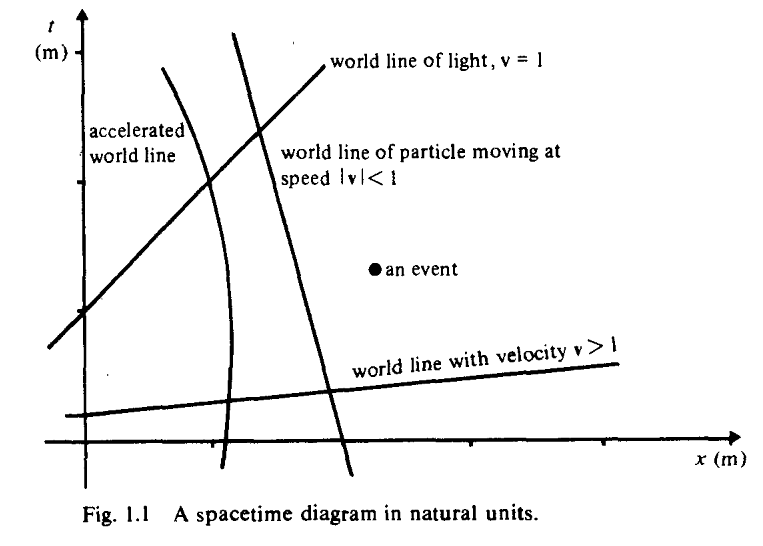
\includegraphics[width=225px]{img/diagram1.png}
    \end{center}
    \[\text{slope}=\frac{dt}{dx}=\frac{1}{v}\]
\end{frame}

\begin{frame}
    \frametitle{The geometry of Newtonian mechanics}
    In Newtonian mechanics we ``consider all of space at a single moment in time.''
    This allows us to think about the geometry of space as independent of motion:
    \begin{align*}
        \Delta s_N^2&=(\Delta x)^2+(\Delta y)^2\\
        &=(\Delta x')^2+(\Delta y')^2
    \end{align*}
    \begin{center}
        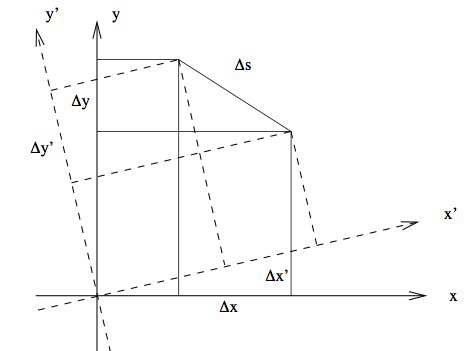
\includegraphics[width=150px]{img/coordchange.png}
    \end{center}
\end{frame}

\begin{frame}
    \frametitle{The geometry of spacetime}
    \begin{block}{Theorem}
        Under the postulates of special relativity, the \textbf{spacetime interval}
        \[\Delta s^2=-(\Delta t)^2+(\Delta x)^2+(\Delta y)^2+(\Delta z)^2\]
        between two events $\mathbf x$ and $\mathbf x'$ is independent of the inertial frame.
    \end{block}
    \begin{itemize}
        \item Note: the usual Newtonian $\Delta s_N^2$ is no longer invariant
        \item The global geometry of spacetime is 4D, non-Euclidean!
    \end{itemize}
\end{frame}

\begin{frame}
    \frametitle{Light cone}
    \begin{center}
        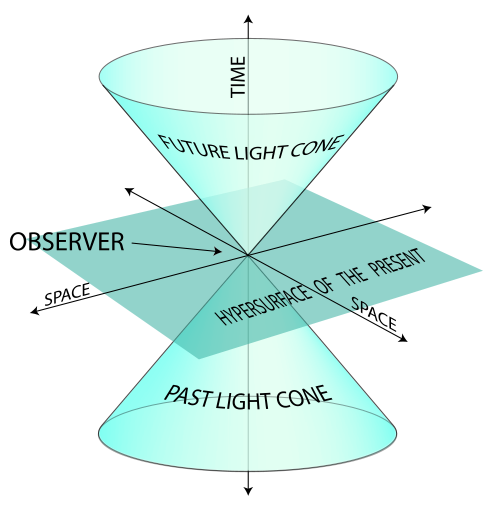
\includegraphics[width=200px]{img/lightcone.png}
    \end{center}
\end{frame}

\subsection{The Lorentz transformations}

\begin{frame}
    \frametitle{Transformation symmetries}
    If inertial observers do not agree on distances and times, what's the conversion rate?
    Equivalently - what transformations leave the spacetime interval unchanged?
    \begin{block}{Question}
        Given two events $\mathbf{x_1},\mathbf{x_2}$, since the spacetime interval
        is a function $\Delta s^2(\mathbf{x_1},\mathbf{x_2})$, we wish to find all such
        (linear) transformations $\Lambda$ such that
        \[\Delta s^2(\mathbf{x_1},\mathbf{x_2})=\Delta s^2(\Lambda\cdot \mathbf{x_1},\Lambda\cdot \mathbf{x_2})\]
    \end{block}
\end{frame}

\begin{frame}
    \frametitle{The Lorentz group}
    \begin{itemize}
        \item The set of such transformations is known as the \textbf{Lorentz group}, $\text{O}(3,1)$,
            and the transformations are known as Lorentz transformations
        \item The Lorentz group was recognized mathematically by Poincar\'e just months before Einstein
            derived them from the postulates of SR
        \item An event $\mathbf{x}$ in on inertial frame will look like $\Lambda\cdot \mathbf{x}$ in another,
            where $\Lambda$ is a Lorentz transformation that depends on the relative orientation and velocity
            of the frames
    \end{itemize}
\end{frame}

\begin{frame}
    \frametitle{Lorentz boost in the $x$-direction}
    Explicitly, one can characterize a Lorentz ``boost'' in the $x$-direction to a frame with relative velocity $v$ as:
    \begin{align*}
        t'&=\gamma(t-vx)\\
        x'&=\gamma(x-vt)\\
        y'&=y\\
        z'&=z\\
        \gamma&=\frac{1}{\sqrt{1-v^2}}
    \end{align*}
    More general transformations rapidly become much more tedious.
\end{frame}

\section{Relativistic effects}
\subsection{Time dilation}

\begin{frame}
    \frametitle{Time dilation}
    Consider a box moving with uniform velocity $\mathbf{v}$ in a lab. Denote by $\mathcal{L}$ the lab frame,
    whose coordinate system is given $(t,x,y,z)$, and $\mathcal{O}$ the frame in which the box is at rest, whose
    coordinate system is given $(\tau,x',y',z')$. We can write:
    \begin{align*}
        -(\Delta \tau)^2&=-(\Delta t)^2+(\Delta x)^2+(\Delta y)^2+(\Delta z)^2\\
        &=-(\Delta t)^2+v^2(\Delta t)^2
    \end{align*}
    and thus
    \[\Delta t=\frac{\Delta \tau}{\sqrt{1-v^2}}=\gamma\Delta \tau.\]
\end{frame}

\begin{frame}
    \frametitle{Time dilation: sanity checks}
    Moving clocks appear to run slower! The lab $\mathcal{L}$ sees its own clock tick $\gamma$ times
    for every once that it sees $\mathcal{O}$'s clock tick.
    \[\Delta t=\gamma\Delta \tau>\Delta \tau\]

    The Newtonian limit $v\to 0$, $\Delta t\to \Delta \tau$ checks out.

    In the extreme relativistic limit $v\to 1$, $\Delta t\to \infty$!
\end{frame}

\subsection{Length contraction}

\begin{frame}
    \frametitle{Length contraction}
    Consider now an observer moving at a velocity $v$ with respect to the box, supressing all but one spatial dimensions.
    Suppose the box has rest length $L_0$ (i.e. $\Delta x'=L_0$). Then
    \begin{align*}
        \frac{L^2}{v^2}&=\frac{L_0^2}{v^2}-L_0^2\\
        L&=L_0/\gamma
    \end{align*}
    In other words, the moving observer find that the length of the box has diminished by a factor of $\gamma$!
\end{frame}

\subsection{Failure of simultaneity}

\begin{frame}
    \frametitle{Failure of simultaneity}
    \url{https://upload.wikimedia.org/wikipedia/commons/7/78/Relativity_of_Simultaneity_Animation.gif}
\end{frame}

%\subsection{``Paradoxes''}
\subsection{SR and modern physics}

\begin{frame}
    \frametitle{Modern physics}
    \begin{itemize}
        \item Special relativity has become a touchstone of modern physics; only those theories consistent
            with relativity may be considered - Lagrangians must be manifestly covariant
        \item SR (and by extension, GR) motivated much interdisciplinary research: mathematical physics is
            now highly geometric (spacetime, bundles) and algebraic (symmetries, representations) in nature
            $\to$ gauge theories like the Standard Model
        \item This has allowed researchers to attack questions in fundamental physics from a variety of perspectives
    \end{itemize}
\end{frame}

\begin{frame}
    \frametitle{References}
    \begin{thebibliography}
        \beamertemplatebookbibitems
        \bibitem{jackson} J.D.~Jackson. \textit{Classical Electrodynamics}, (1999).
        \bibitem{schutz} B.~Schutz. \textit{A course in general relativity}, (2009).
    \end{thebibliography}
\end{frame}


\end{document}

